\documentclass[11pt]{article}
\usepackage[margin=0.78in]{geometry}
\usepackage{amsmath,booktabs,array,graphicx,float,hyperref}
\hypersetup{colorlinks=true,urlcolor=blue,linkcolor=blue}
\setlength{\parindent}{0pt}
\setlength{\parskip}{6pt}
\newcommand{\smalltitle}[1]{\vspace{5pt}\textbf{#1}\par}
\begin{document}
\begin{center}
{\Large Assignment 7: Fund X and the Two Regime Model}\\[5pt]
Prepared by Harman Singh for Professor Phelim Boyle\\
September 2026
\end{center}

\smalltitle{What the model tells us}
The two-regime idea suits Fund X because its returns change in both size and
variability. Many months have modest gains, while other periods contain much
larger gains. Letting the fund move between two return patterns describes that
history better than forcing every month into one distribution.

The supplied note's exact fit is not the best one found. A fresh fit, independently
checked with a second implementation, raises the log-likelihood from the reported
255.75 to \textbf{261.11}. It describes a quieter state averaging \textbf{1.55\%}
per month and a more variable state averaging \textbf{5.68\%}. Both last about
13 months on average. That differs substantially from the note's short, two-month
bursts averaging 9.6\%.

\smalltitle{Why that is economically plausible}
The fund's factsheet describes a systematic long/short equity strategy with low
net market exposure. Trading opportunities could change over time even when the
overall market direction is unhelpful. Two positive-mean states are consistent
with that description. Returns alone do not establish the trading mechanism,
manager skill, or the accuracy of reported valuations. The model is useful for
describing varying return conditions and building conditional scenarios.

\smalltitle{What was checked and why}
All 115 returns from January 2017 through July 2026 match the saved source
factsheet exactly. There are five negative months; the mean is 3.52\% and the
sample standard deviation is 3.98\% per month. July is marked estimated.
The comparison keeps this date range fixed.

\begin{table}[H]\centering\small
\caption{Allowing two distributions produces most of the improvement}
\begin{tabular}{lrrrr}\toprule
Model & Parameters & Log-likelihood & AIC & BIC\\\midrule
One regime & 2 & 217.17 & -430.34 & -424.85 \\
Independent mixture & 5 & 256.91 & -503.82 & -490.10 \\
Two regimes stationary & 6 & 261.11 & -510.22 & -493.75 \\
Two regimes free initial & 7 & 261.39 & -508.78 & -489.56 \\
\bottomrule\end{tabular}
\end{table}
An independent mixture allows two distributions but redraws the state each month.
It already beats the note's reported likelihood. Adding persistence improves
the refitted model further. Lower AIC and BIC favor the improved switching fit,
but these are model comparisons, not proof of a unique economic explanation.

\begin{table}[H]\centering\small
\caption{The interpretation changes when the model is refitted}
\begin{tabular}{lrrrr}\toprule
State & Mean return & Return SD & Duration (months) & Long-run share\\\midrule
Note ordinary & 2.42\% & 2.16\% & 11.4 & 84.2\% \\
Note high & 9.56\% & 6.65\% & 2.1 & 15.8\% \\
Improved lower & 1.55\% & 1.16\% & 13.7 & 50.7\% \\
Improved higher & 5.68\% & 4.58\% & 13.3 & 49.3\% \\
\bottomrule\end{tabular}
\end{table}
\newpage

\smalltitle{The high state is more than a handful of exceptional months}
\begin{center}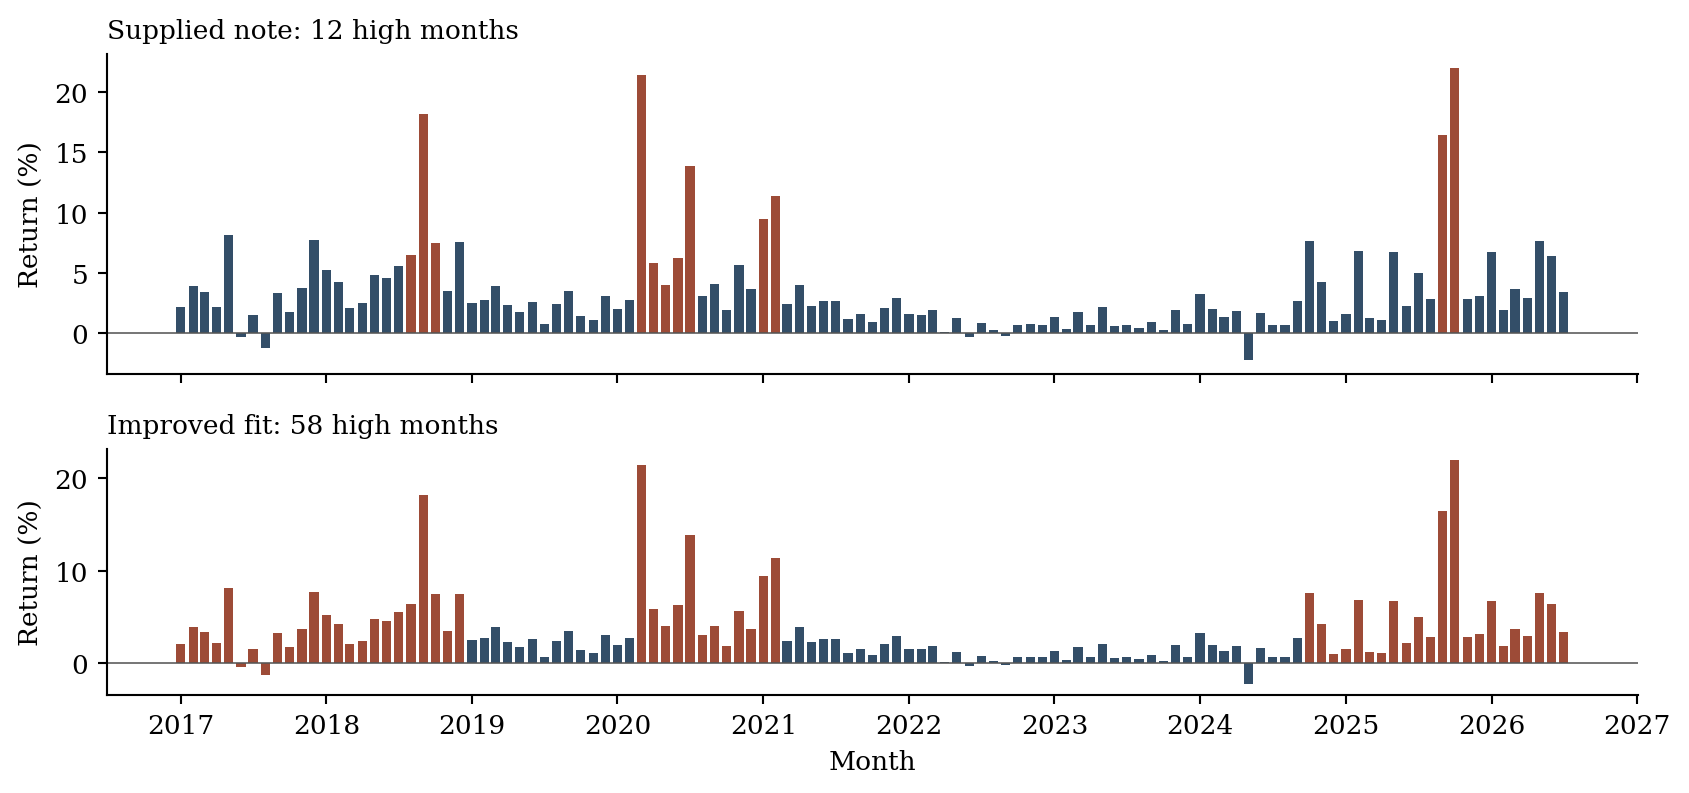
\includegraphics[width=.98\linewidth]{figures/regime_comparison.png}\end{center}
\small Red bars mark the higher-return state on the most likely full-sample
path. These labels use hindsight. They are not signals available before each
month. Long-run state shares in the table are different from observed path counts.
\normalsize

\smalltitle{The tests and what they mean}
\textbf{Does the order of months matter?} Yes. Shuffling the same 115 returns
499 times and refitting produces an equal or larger switching-versus-mixture
gain only twice (one-sided Monte Carlo $p=0.006$). Timing contains information
beyond the return histogram. This rejects exchangeable ordering; gradual changes
or other dependence could also produce that finding.

\textbf{Does the model explain the rare losses?} Only partly. The note's fitted
distribution expects about \textbf{13.9} loss months out of 115; the improved
fit expects \textbf{11.2}. Only \textbf{five} occurred. A positive mean in each
state does not remove the negative tail. Neither model shows that future losses
will remain rare or small.

\textbf{Is dependence left over?} Raw lag-one autocorrelation is 0.352.
Predictive innovations from the improved fit have lag-one autocorrelation 0.156.
Their 12-lag statistic is 19.70; a bootstrap that simulates and refits the model
gives $p=0.080$ (199 simulations). This does not reject at 5\%, but it also does
not establish independence or correct tail behavior.

\begin{table}[H]\centering\small
\caption{One-month-ahead checks from January 2025 through July 2026}
\begin{tabular}{lrr}\toprule
Model & Total log predictive score & Mean forecast RMSE\\\midrule
One regime & 24.15 & 5.66\% \\
Independent mixture & 32.99 & 5.66\% \\
Switching model & 26.90 & 5.49\% \\
\bottomrule\end{tabular}
\end{table}
Higher log scores mean better predictions of the whole return distribution;
lower RMSE means smaller errors in the predicted mean. The switching model has
slightly lower mean error, but the simpler mixture has the best distribution
score. Each forecast uses only earlier returns. This is a retrospective check
of 19 months, with the model family chosen after seeing the full history, so it
does not establish a reliable trading advantage.
\newpage

\smalltitle{Short technical notes}
\textbf{Model and units.} Monthly simple returns are decimals, net of management
and performance fees for the source's I series. With $y_t=\log(1+r_t)$,
$y_t\mid S_t=i\sim N(\mu_i,\sigma_i^2)$, and the two-state transition matrix is
row-stochastic. The primary likelihood starts in its stationary distribution.
The mean simple return is $e^{\mu_i+\sigma_i^2/2}-1$; expected duration is
$1/(1-p_{ii})$. All reported likelihoods use log-return density. Converting to
simple-return density subtracts $\sum_t\log(1+r_t)$ from every likelihood, so
model rankings and likelihood differences are unchanged. No annualization is used.

\textbf{Optimization and reproduction.} The primary search uses 300 starts,
EM starting values, and direct constrained likelihood maximization. A separate
\texttt{statsmodels} Hamilton-filter fit agrees within $10^{-5}$ log-likelihood
units. The standard deviation floor is 0.001 in log-return units; halving and
doubling it leaves the main result unchanged. The fitted standard deviations
are far above this floor. A floor avoids a component collapsing onto one
observation, where an unrestricted Gaussian-mixture likelihood can diverge.
This is the best nondegenerate fit found, not a proof of a global maximum.

\textbf{Corrections to the supplied note.} Its one-regime likelihood, raw ACF,
12 high-month labels, and regime-demeaned lag-one ACF of 0.157 reproduce. Using
its rounded parameters gives likelihood 255.56 with its stated rounded
stationary weights, or 255.71 if the first month is fixed in the lower state.
The original code, unrounded parameters, and initialization were not supplied,
so the exact source of the reported 255.75 and stopping rule cannot be verified.
In either case, better fits exist. Six parameters versus two means
\textbf{four}, not three, extra parameters. Estimating the initial-state weight
adds a seventh parameter. A usual chi-square likelihood-ratio reference is
invalid when states become indistinguishable under the null. The note correctly
recognizes nonregularity, but its one-regime comparison alone cannot isolate
the contribution from persistence.

\textbf{Residual and tail interpretation.} Subtracting full-sample Viterbi state
means uses hindsight and leaves different variances across states. Its ordinary
Ljung--Box p-values are descriptive, without a valid automatic correction for
estimated states. The alternative check uses
$z_t=\Phi^{-1}\{\sum_i w_{t|t-1,i}\Phi[(y_t-\mu_i)/\sigma_i]\}$ and refits
every bootstrap sample. The model-implied probabilities of at most five losses
are 0.0040 for the note and 0.0286 for the improved fit, computed by an exact
Markov count recursion at fixed fitted parameters. These are predictive
calibration warnings, not exact goodness-of-fit p-values after estimation.

\textbf{Stability.} Removing estimated July leaves mean returns near 1.55\%
and 5.75\%, with durations near 13 months. Returning to the earlier May sample
gives 1.57\% and 5.83\%. Hiding each of four high-return episodes, while preserving
calendar transitions, leaves two positive-mean patterns but can materially change
their durations. The January--February 2021 deletion gives approximately
6.7 and 2.9 months. Precise state labels and durations should therefore
be treated as sample-sensitive estimates.

\smalltitle{Connection to prior work and sources}
This extends Assignment 3's serial-dependence question on the longer July sample.
It supports examining changing return conditions, but does not identify their
cause or prove the absence of smoothing. Assignment 3 used 113 observations to
May; this note uses 115 to July.

{\footnotesize
Source: supplied \texttt{Fund\_X\_two\_regime\_model.docx}, September 2026.
The stated \texttt{COMBined3b.xlsx} was not found. The project CSV
was instead independently reconciled month by month to the saved
\href{https://spartanfunds.ca/wp-content/uploads/2021/11/LSQ-Oct21.pdf}{July 2026 fund factsheet},
downloaded August 10, 2026; its exact snapshot and hash are retained.\\
Method references: Hardy (2001), \emph{North American Actuarial Journal} 5(2),
41--53, bibliographic details checked against the
\href{https://uwaterloo.ca/statistics-and-actuarial-science/profiles/mary-hardy}{author's university profile};
\href{https://www.statsmodels.org/stable/examples/notebooks/generated/markov_regression.html}{statsmodels Markov switching documentation};
\href{https://scikit-learn.org/1.0/modules/mixture.html}{scikit-learn Gaussian mixture documentation}.
}
\end{document}
